
% Chapter 3

\chapter{État de l'art} % 3rd chapter title

\label{Chapter3} % For referencing the chapter elsewhere, use \ref{Chapter3} 


%----------------------------------------------------------------------------------------

\section{Position du problème}

\subsection{Modélisation d'un floe de glace}

Nous commensons par présenter une modélisation mathématique d'une plaque de glace (appelé floe) sur la mer. Six variables (locales) sont nécésaires pour décrire un floe sur la mer (voir figure 1): 
\begin{itemize}
    \item Un ouvert connexe $\omega \in \Rdeux$ décrivant la section longitidunale du floe;
    \item Deux fonction $\hplus, \hmoins \in \mathcal{F}(\omega, \Run)$ décrivant l'épasseur du floe, telle que $\forall x \in \omega, \hmoins(x) \leq \hplus(x)$;
    \item Le centre de gravité du floe $G(w)$;
    \item Deux vecteurs $e_1(\omega)$ et $e_2(\omega)$ formant une base sur $\omega$.
\end{itemize}

\begin{figure}[H]
    \centering
    \begin{subfigure}[b]{0.45\textwidth}
        \centering
        % 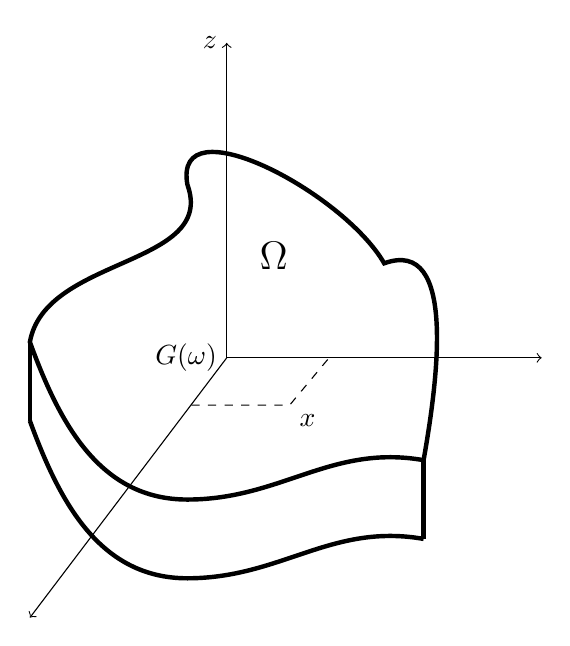
\begin{tikzpicture}
\node[coordinate] (v1) at (-3,3) {};
\node[coordinate] (v2) at (-5,1) {};
\node[coordinate] (v3) at (-3,-1) {};
\node[coordinate] (v4) at (0,-0.5) {};
\node[coordinate] (v5) at (-0.5,2) {};
%\draw  plot[smooth cycle, tension=.7] coordinates {(v5) (v1) (v2) (v3) (v4) (v5)};

\draw [ultra thick] (v1) to [out=290, in=80] (v2) to[out=290, in=180] (v3) to[out=0,in=170] (v4) to[out=80,in=20] (v5) to[out=120,in=100] (v1);

\node[coordinate] (v6) at (-5,0) {};
\node[coordinate] (v7) at (-3,-2) {};
\node[coordinate] (v8) at (0,-1.5) {};

\draw [ultra thick] (v2)--(v6); \draw [ultra thick] (v4)--(v8);
\draw [ultra thick]  (v6) to[out=290, in=180] (v7) to[out=0,in=170] (v8);

\node[coordinate] (v9) at (-2.5,0.8) {};
\node[coordinate] (v10) at (-5.0,-2.5) {};
\node[coordinate] (v11) at (1.5,0.8) {};
\node[coordinate] (v12) at (-2.5,4.8) {};

\draw [->] (v9)--(v10);
\draw [->] (v9)--(v11);
\draw [->] (v9)--(v12);


\node[left] (v9) at (-2.5,0.8) {$G(\omega)$};
\node[left] (v12) at (-2.5,4.8) {$z$};
\node[above left] (v13) at (-1.6,1.8) {\Large $\Omega$};

\node[coordinate] (v14) at (-1.2,0.8) {};
\node[coordinate] (v15) at (-1.7,0.2) {};
\node[coordinate] (v16) at (-2.95,0.2) {};
\draw[dashed] (v16)--(v15)--(v14);

\node[below right] (v15) at (-1.7,0.2) {$x$};

\end{tikzpicture}

        \includegraphics[width=.8\textwidth]{FloeVue1.tikz} 
        \caption{Vue d'un floe}
        % \label{fig:floe1}
    \end{subfigure}
    % \hfill
    \begin{subfigure}[b]{0.45\textwidth}
        \centering
        % \usetikzlibrary{patterns}

\begin{tikzpicture}

\node[coordinate] (v0) at (0,0) {};
\node[coordinate] (v1) at (-5,0) {};
\node[coordinate] (v2) at (5,0) {};
\node[coordinate] (v3) at (0,-5) {};
\node[coordinate] (v4) at (0,5) {};

\draw [->] (v1)--(v2);
\draw [->] (v3)--(v4);

\node (v5) at (-4,2.5) {};
\node (v6) at (-1.5,3.5) {};
\node (v7) at (1,3.5) {};
\node (v8) at (3,2.5) {};
\node (v9) at (4,2.5) {};
\node (v10) at (-3.5,-2.5) {};
\node (v11) at (-2,-3.5) {};
\node (v12) at (-0.5,-3) {};
\node (v13) at (0.5,-3) {};
\node (v14) at (2,-3.5) {};
\node (v15) at (4.5,-3.5) {};

\draw[ultra thick]  plot[smooth, tension=.7] coordinates {(v5) (v6) (v7) (v8) (v9)};
\draw[ultra thick]  plot[smooth, tension=.7] coordinates {(v10) (v11) (v12) (v13) (v14) (v15)};

\draw [white, pattern=north east lines, xshift=0.5cm,yshift=4.5cm] plot coordinates {(v5) (v6) (v7) (v8) (v9) (v15) (v14) (v13) (v12) (v11) (v10) (v5)};

\node [above right] at (0,3.5) {\Large \bfseries $h_{+}(x)$};
\node [below right] at (0,-3.5) {\Large \bfseries $h_{-}(x)$};
\node [right] at (5,0) {\Large \bfseries $x$};
\node [left] at (0,5) {\Large \bfseries $z$};

\end{tikzpicture} 
        \includegraphics[width=.8\textwidth]{FloeVue2.tikz} 
        % \includegraphics[width=2cm]{Figures/FloeVue2.tex}
        \caption{Coupe transversale}
        \label{fig:flo2}
    \end{subfigure}
       \caption{Illustration de la géométrie d'un floe de glace $\Omega$.}
       \label{fig:floe}
\end{figure}

\emph{LES VECTEURS E1 ET E2 (ET TOUS LES AUTRES VECTEURS) DOIVENT ETRE EN GRAS !}

Le volume $\Omega$ du floe est donné par:
\[
    \Omega = \{(x,z) | x \in \omega \in \Rdeux, z \in ]\hmoins(x), \hplus(x)[ \} \,.
\] 
Les fonctions $\hmoins$ et $\hplus$ permettent de définir trois quantités (voir figure 2):
\begin{itemize}
    \item L'épaisseur moyenne du floe : $\bar{h} =  \sup_{x\in\omega}{\hplus(x)} - \inf_{x\in\omega}{\hmoins(x)}$;
    \item La plus forte epaisseur : $\bar{h}^* = \sup_{x\in\omega}{ \vert \hplus(x) - \hmoins(x) \vert}$. 
    \item La plus faible epaisseur : $\underline{h}^* = \inf_{x\in\omega}{ \vert \hplus(x) - \hmoins(x) \vert} $. 
\end{itemize}

\begin{figure}
    \centering
    % \input{Figures/Epaisseur.tikz}
    \includegraphics[width=.6\textwidth]{h.tikz}
    \caption{Illustration des différentes épaisseurs décrivant le floe de glace. Pour l'instant, afin d'obtenir un floes relativement plat (i.e $\bar{h}$ faible), $\hmoins$ sera pris identiquement nul, et $\hplus$ constant.}
\end{figure}

Les vecteur $e_1(\omega)$ et $e_2(\omega)$ sont liés à $\omega$, et pointent vers un point fixe du bord $\partial \omega$ du floe i.e:
\[
    \exists \sigma_i \in \partial \omega | e_i(\omega) = \frac{\sigma_i - G(\omega)}{\Vert \sigma_i - G(\omega) \Vert}, \text{ pour } i \in \{1,2\} \,,
\]
où $\Vert \cdot \Vert$ désigne la norme euclidienne de $\Rdeux$. Notons que $\sigma_1 \neq \sigma_2$, et $\eun \cdot \edeux = 0$ de facon à ce que la base $(\eun, \edeux)$ soit directe.

Un floe $F = (\omega, \eun, \edeux, G(\omega), \hmoins, \hplus)$ se déplace sur la mer\footnote{Pour l'instant, la mer est considérée comme un ouvert dans $\Rdeux$. Plus tard, nous prendrons en compte sont épaisseur lorsque nous la modelserons par une sphère} $\mathcal{M} \in \Rdeux$. Au temps $t$ après une translation de vecteur $u(t)$ (et de matrice $\mathsf{T}_{u(t)}$), et une rotation de vecteur $\theta(t)$ (et de matrice $\bmat{R}_{\theta(t)}$), on obtient le floe $F_t$ défini par (voir figure 3):
\[
    F_t = (\mathsf{T}_{u(t)}\mathsf{R}_{\theta(t)}\omega, T_{u(t)}R_{\theta(t)}\eun, T_{u(t)}R_{\theta(t)}\edeux, T_{u(t)}R_{\theta(t)}G(\omega), \hmoins, \hplus) \,.
\]
\emph{REMPALCER CES TRANSFORMATION ENCOMBRANTES PAR UN prime SIMPLE !}

\begin{figure}[!h]
    \centering
    % \input{Figures/Epaisseur.tikz}
    \includegraphics[width=.4\textwidth]{FloeMer.tikz}
    \caption{Illustration du mouvement d'un floe de glace $F$ dans la mer, après une translation de vecteur $u(t)$ et une rotation d'angle $\theta(t)$, pour obtenir le floe $F_t$. On observe la transformation des propriétés du floe, en partucilier les vecteurs $e_1(\omega)$ et $e_2(\omega)$ qui restent liés au floe.}
\end{figure}


Lors de leur mouvements sur la surface de la mer, les floes se fracturent sous l'effet des vents et des courants océaniques. Nous nous interreserons donc au phénomène de percussion en vue de l' initialisation des fractures dans les floes de glace. 


Afin de décrire le mouvement des floes de glace sur la mer, nous devons nous munir d'un repère abosulu, que notons $\mathcal{R}_{abs} = (O, \bm i, \bm j, \bm k)$. le repère associé au floe $\Omega_i$ sera noté $\mathcal{R}_{\Omega^i} = (O, \bm \eun, \bvec \edeux, \bvec k)$. Dans ce repere absolu, le floe possède 3 dégrés de libertés: l'absice et l'ordonné de son centre de gravité $G^i(\omega)$, et l'orientation du floe donné par l'angle $\theta^i (t)$ (voir \cref{fig:FloeRepere}). 

\begin{figure}[!h]
    \centering
    % \input{Figures/Epaisseur.tikz}
    \includegraphics[width=.5\textwidth]{FloeRepere.tikz}
    \caption{Positionnement d'un floe de glace $\Omega^i$ dans le repère absolu $\mathcal{R}_{abs}$.}
    \label{fig:FloeRepere}
\end{figure}


\textit{DEFINIR LE REPERE aBSOLUE DU FLOE EN 2D, AVEC LE REPERE LOCAL. ECRIRE LE VECTEUR POSITION, ET ECRIRE LES EQUATIONS DE NEWTON-EULER.}





%----------------------------------------------------------------------------------------
\section{État de l'art}

Une fois le modèle défini, il nous faut établir les équations décrivant la dynamique du floe, et celle de son environnment. Les travaux de \cite{rabatel2015thesis} et \cite{balasoiu2020thesis} on extensivement traité le problème de modélisation dynmaique et de simulation d'un assemblage de floe cde glace. Nous résumons ici les principales idées de leurs raisonnements, tout en présentant l'état de l'art dans ce domaine.

\subsection{Le modèle du floe}

\subsubsection{La cinetique du floe}

L'approche discrète décrite dans \parencite{rabatel2015thesis} consiste a définir le mouvement de chaque floe. Les obstacles sont des floes aux mêmes propriètés que les floes de galce, à la seule différence qu'ils ont une masse (volumique) infinie. Dans \parencite{rabatel2015thesis}, l'auteur travaille dans un repère orthormé direct $\mathcal{R}_{abs} = (O, \bm i, \bm j, \bm k)$, cependant, la mer est considérée plane, et le mouvement du floe peut être décrit dans le plan $\mathcal{P} = (O, \bm i, \bm j)$. On désigna la vitesse angulaire du floe $\Omega^i$ par 
$$
\bvec{\uptheta}^i(t) = \theta^i(t)\bvec{k} = (0,0,\theta^i(t))^T \,.
$$
Soit $P$ de coordonné $x$ un point quelconque de $\P \subset \Rdeux$. Sa vitesse dans le repère $\R_{abs}$ est donnée est donnée par la formule de Varignon:
$$
\dot{P}(t) = \dot{G}^i(t) + \bm{\uptheta}^i(t) \wedge \bvec{G^iP} \,,
$$
où le symbole $\wedge$ représente le produit vectoriel dans $\Rtrois$. La masse (constante) du floe rigide indéformable est donnée par 
$$
M^i = \rho^i \int_{\Omega^i(t)} \hplus^i (x) \diff x \,.
$$
Ensuite, l'auteur défni :
\begin{itemize}
    \item la somme des force par unité de volume qui s'applique au centre de masse du floe $\Omega^i$: $$\bvec{F}^i = \rho^i \int_{\Omega^i(t)} \bvec{F}(x) dx \,.$$
    \item le moment cinetique\footnote{du à l'accélération du floe} en $G$: $$L^i = \rho^i \intO{i} \bvec{GP} \wedge \dot{\bvec{P}}(t) \diff x \,.$$
    \item le moment dynamique\footnote{du aux forces extérieurs exercées sur le floe} en $G$: $$\bvec{\mathfrak{M}}^i = \intO{i} \bvec{GP} \wedge \bvec{F}(x) \diff x \,.$$
\end{itemize}
Sous le formalisme de Newton-Euler, \citeauthor{rabatel2015thesis} montre que chaque floe $\Omega^i$ vérifie:
$$
% \begin{align}
    \begin{cases}
        M^i \frac{\diff \dot{\bvec{G}}^i(t)}{\diff t} &= \bvec{F}^i \\
        \mathcal{I}^i \frac{\diff \dot{\bvec{\uptheta}}^i(t)}{\diff t} &= \bvec{\mathfrak{M}}^i
    \end{cases} \,,
% \end{align}
$$
qui se réecrit facilement sous la forme 
\begin{align}    
    \mathcal{M}^i \frac{\diff W^i(t)}{\diff t} = \mathcal{H}^i(t) \,,
\end{align}
avec 
$$
\mathcal{M}^i = 
\begin{pmatrix}
    M^i & 0 & 0 \\ 0 & M^i & 0 \\ 0 & 0 & \mathcal{I}^i
\end{pmatrix} \,,
W^i(t) = 
\begin{pmatrix}
    \dot{\bvec{G}}(t) \\ \dot{\theta}^i(t)
\end{pmatrix} \,
\text{et } \mathcal{H}^i(t) = 
\begin{pmatrix}
    \bvec{F}^i(t) \\ \mathfrak{M}^i(t)
\end{pmatrix} \,.
$$
Pour un système composé de $n$ floes, l'équation précédente doit être satisfaite pour tous les floes. \cite[p.18]{rabatel2015thesis} montre que cela revient au système d'équations
\begin{align} \label{eq:bilan1}
    \mathcal{M} \frac{\diff W(t)}{\diff t} = \mathcal{H}(t) \,,
\end{align}
avec 
$$
\mathcal{M} = (\mathcal{M}^i)_{1\leq i \leq n } \,,
\mathcal{W}(t) = (\mathcal{W}^i(t))_{1\leq i \leq n } \, \text{et }
\mathcal{M}(t) = (\mathcal{M}^i(t))_{1\leq i \leq n }  \,.
$$
L'énergie cinétique du floe $\Omega^i$ quant à elle sera donné par:
$$
E^i(t) = \frac{1}{2}M^i \dot{G}^i(t)^2 + \frac{1}{2}\mathfrak{I}^i \dot{\theta}^i(t)^2 \,. 
$$ 



\subsubsection{L'interaction entre les floes}

Le domaine de la mécanique du contact s'est grandemen développé ces dernier siècles, avec plusieurs scientifique qui ont tenté de décrire décrire le phénomène de contact entre des coprs. Le modèle décrit par \parencite[p.5892]{rabatel2015dynamics} utilise deux conditions de complémentarité pour déterminer les vitesses des floes après le contact. 

La primière est une condition de Signorini\parencite{signorini1933sopra} pour s'assurer de la non-interpénétration\footnote{Deux floes s'interpénètre si la "distance" entre ces deux floes est négative.} des floes. Pour écrire ces conditions, il faut au préalable écrire le problememe de contact entre floes comme un problème implcite, où les inconnus sont les impulsions après le choc. \citeauthor{rabatel2015thesis} se base donc sur les travaux de Delassus (1917), Moreau (63), (Pfeiffer and Glocker, 1996), [Stewart and Trinkle, 1996; Stewart, 2000; Anitescu and Potra, 1997; Anitescu et al., 1999]. Dans \parencite[p.5892]{rabatel2015dynamics}, le problème de complémentarité a ensuite résolu en utlisant l'algorithme de Lemke [Cottle et al., 1992, Alg. 6.3.1]. 

\textit{IMAGE D'UNE COLLISION EN Pj}

Soit $P_j$, ($j \in \{1,\ldots,n\}$) un point de contact entre les floes $\Omega_k$ et $\Omega_l$. Nous notons $\bvec{F}_{kj}(t)$ la force de contact du floe $\Omega_k$ au floe $\Omega_l$ appliquée en $P_j$. Par convention, une matrice de contact $\bmat{M_c}$ est définie telle que son coefficient $c_kj$ vaut:
\begin{itemize}
    \item $0$ si le point de contact $P_j$ n’est pas un point de contact du floe $\Omega_k$;
    \item $-1$ si le point de contact $P_j$ est un point de contact entre les floes $\Omega_k$ et $\Omega_l$ avec $k < l$;
    \item $1$ si le point de contact $P_j$ est un point de contact entre les floes $\Omega_k$ et $\Omega_l$ avec $k > l$.
\end{itemize}
En notant $E_k$ l’ensemble des points de contact du floe $\Omega_k$ au temps t, \parencite[p.26]{rabatel2015thesis} définit la résultante des forces de contact $\bvec{F}^c_k(t)$, au floe $\Omega_k$ comme :
$$
\bvec{F}^c_k(t) = \sum_{j \in E_k} c_{jk} \bvec{F}_{kj}(t) 
$$
En rajoutent ces forces aux forces extérieures lors du bilan des forces à l'\cref{eq:bilan1}, on obtient, pour un floe $\Omega_k(t)$ :
\begin{align} \label{eq:bilan1}
    \mathcal{M} \frac{\diff W(t)}{\diff t} = \mathcal{H}(t) + \sum_{j \in E_k} \begin{pmatrix}
        \bvec{F}_{kj}(t) \\ \bvec{G^kP_j} \wedge \bvec{F}_{kj}(t) 
    \end{pmatrix} \,.
\end{align}


\subsubsection{Formulation en problème linéaire de complémentarité}

Il existe deux principales manières de formuler le problème du contact entre deux solides rigides. L'auteur de \parencite{rabatel2015thesis} opte pour le formulisme vitesse-impulsion, au détriment du formalisme accéleration-force. En effet, L’approche en vitesse impulsion apporte donc l’avantage de pouvoir exprimer la force de friction de Coulomb directement par rapport à la vitesse. Il n’est pas nécessaire de connaître la nature du contact. 
Il nous faut donc définir les notions d'impulsion. Sur un intervalle de temps $\delta t^*$, s’il y a un contact au point $P_j$, entre les floes $\Omega_k$ et $\Omega_l$, nous dirons que le floe $\Omega_k$ a subi un choc provenant du floe $\Omega_l$ au point de contact $P_k$ caractérisé par l’impulsion :
$$
\bvec{\mathcal{I}}_{kj} = \int_{\delta t^*} c_{kj} \bvec{F}_{kj}(t) \diff t \,.
$$ 
\citeauthor{rabatel2015thesis} fait donc apparaître les impulsions dans les équations des moments \cref*{eq:bilan1} pour le floe $\Omega_k$ sur l’intervalle temporel $\delta t^*$:
$$
\mathcal{M}_k \int_{\dtstar} \dot{W}_k(t) \diff t = \int_{\dtstar} \mathcal{H}(t) \diff t + \sum_{j \in E_k} \begin{pmatrix}
    \bvec{\mathcal{I}}_{kj} \\ \bvec{G_kP_j} \wedge \bvec{\mathcal{I}}_{kj} 
\end{pmatrix} \,.
$$
En écrivant $\dtstar = [t^{-}, t^{+}]$, on peut donc introduire les inconnues $\beta$, $\lambda \in (\Rdeux)^m$ pour le problème de contact  
\begin{align}
    \mathcal{M}_k \left( W(t^{+}) - W(t^{-}) \right) = \int_{\dtstar} \mathcal{H}(t) \diff t + \bmat{B}\beta + \bmat{J}\lambda \,,
\end{align}
où $\bmat{B}$ sont deux matrices telle que \dots (equation 1.1.14 de la these)

Il devient posible de formuler le problème de contact sans interpénétration par un problème lineaire de complémentarité:
(equation 1.1.22) de la these

\subsubsection{Conservation de l'énergie cinétique}

\subsubsection{Traitement des conditions aux bords}

\subsection{Le modèle de l'environment}



